
\subsection{\label{sec:example:3dhex8-dike}Dike Intrusion Example}

PyLith features discussed in this tutorial:
\begin{itemize}
\item Fault opening via prescribed tractions to mimic a dike instrusion
\item Dirichlet boundary conditions
\item Elastic material
\item VTK output
\end{itemize}

\subsubsection{Overview}

This set of examples describes a problem where prescribed tensile
tractions are imposed on a fault to mimic a dike intrusion. The example
is contained in the directory \texttt{examples/3d/hex8}, and the corresponding
\texttt{.cfg} file is \texttt{step20.cfg}. The example may be run
as follows:
\begin{lyxcode}
pylith~step20.cfg
\end{lyxcode}
This will cause PyLith to read the default parameters in \texttt{pylithapp.cfg},
and then override or augment them with the additional parameters in
the \texttt{step20.cfg} file. The \texttt{.cfg} file is extensively
documented, to provide detailed information on the various parameters.


\subsubsection{Step20 - Static Dike Intrusion}

The \texttt{step20.cfg} file defines a problem with spatially varying
tensile normal tractions on the fault surface associated with a fluid
intrusion. The lateral sides and bottom of the domain are fixed using
Dirichlet (roller) boundary conditions. As in the other examples,
we also setup output for the ground surface.

We use the FaultCohesiveDyn object to impose tractions on the fault
surface. We must include a fault constitutive model so we choose static
friction with a coefficient of friction of 0.1. The coefficient of
friction is irrelevant for the center of the fault where we impose
uniform tensile tractions (10 MPa) and the fault opens, but it facilitates
clamping the edges of the fault via compressive normal tractions (-100
MPa). Note that we must set the property \texttt{open\_free\_surface}
to False in order for the tractions to be imposed when the fault is
open; the default behavior for fault opening is a free surface (the
two sides of the fault are completely uncoupled). The most important
fault parameters for prescribing the tensile fault tractions are
\begin{lyxcode}
{[}pylithapp.timedependent.interfaces.fault{]}

open\_free\_surface~=~False~\\


traction\_perturbation~=~pylith.faults.TractPerturbation~\\


{[}pylithapp.timedependent.interfaces.fault.traction\_perturbation{]}

db\_initial~=~spatialdata.spatialdb.SimpleDB

db\_initial.label~=~Initial~fault~tractions

db\_initial.iohandler.filename~=~spatialdb/tractions\_opening.spatialdb

db\_initial.query\_type~=~nearest~
\end{lyxcode}
When we have run the simulation, the output VTK files will be contained
in \texttt{examples/3d/hex8/output} (all with a pvrefix of \texttt{step20}).
Results using ParaView are shown in Figure \vref{fig:step20-disp}.

\begin{figure}
\begin{centering}
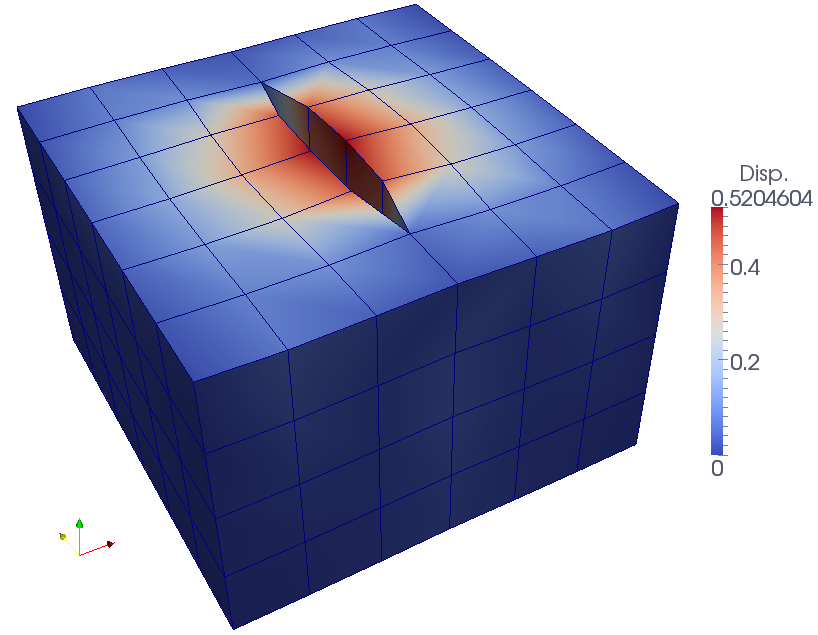
\includegraphics[width=10cm]{tutorials/3dhex8/figs/step20_disp}
\par\end{centering}

\caption{Displacement magnitude for example step20 visualized using ParaView.
\label{fig:step20-disp}}
\end{figure}

